\chapter{图的最优化问题和贪婪算法}\label{Sec:Chap8}
\section{概述}
本章中,我们将学习许多图的可以被贪婪算法精确解决的最优化问题。典型的,
在最优化问题中需要做一系列的选择,以取得最小的消耗,或者得到最大的收益。
贪婪方法由一系列选择组成,每一个单独的选择都使结果向“短期”
\footnote{译注:局部的}最优解靠近,通常局部最优解不需要很多花费
就可以得到。一旦作出了一个选择,它不能被撤销,即使都后面发现它其实
是一个糟糕的选择。由于这个原因,贪婪算法对很多问题不能找到精确的最优解。
但是,对于本章讨论的问题我们可以证明\emph{适当的}贪婪策略会产生
最优的解决方案。在第\ref{Sec:Chapter:NPCompleteProblem}章中,我们将看到
非常类似的贪婪方法无法得到一些问题的解。在
第\ref{Sec:Chapter:DynamicProgramming}章中我们也将看到一些贪婪方法不能
解决的问题。

本章首先给出一个无向图中找最小生成树的算法,由R.C.Prim给出;一个很相关的
在有向和无向图中找最短路径的算法,由E.W.Dijkstra给出;以及第二个找最小
生成树的算法,由J.B.Kruskal给出。所有的算法使用优先权队列来从候选集合中
选择当前最好的选择。

\section{Prim's 最小生成树算法}\label{Sec:PrimMST}
我们学习的第一个问题是找出一个连同的,带权的,无向图中最小生成树。对于
非连同图,该问题的一个自然扩展是找出每一个连同分量的最小生成树。我们
在7.4.2小节看到,连通分支可以在线型时间内找到。

最小生成树仅对无向带权图有意义,所以本小节虽有的“图”都指“无向图”,
权都是边的权。复习符号$G=(V, E, W)$,$W$是一个函数,它给$E$的每一个边
赋予一个权。这仅是数学上的描述。在实现中,一般没有“函数”;每一条边
的权简单的存储在边的结构里面。


\subsection{最小生出树的定义和例子}
\begin{definition}
最小生成树

连通无向图G=(V,E)的最小生成树是G的一个子图,它是一颗无向树且包含G的
所有顶点。在带权图G=(V,E,W)上,子图的权是子图所有边的权的和。带权无向图
的最小生成树(简写为MST)是权最小的生成树。
\end{definition}

\begin{figure*}[!t]
    \centering
    \subfloat[]{
        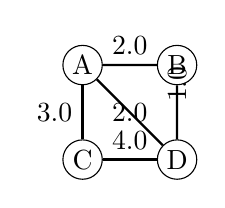
\begin{tikzpicture}[scale=0.6,place/.style={circle,draw, fill=white,inner sep=0pt,minimum size=5mm}]
        \node (x31)  at (2,2) [place] {B};
        \node (x21)  at (2,0) [place] {D};
        \node (x22)  at (0,0) [place] {C};
        \node (x11)  at (0,2) [place] {A};

        \draw [thick] (x31) -- (x21)
            node[midway,sloped,right]{1.0};
        \draw [thick] (x21) -- (x22)
            node[above,text centered,midway]{4.0};
        \draw [thick] (x22) -- (x11)
            node[left,text centered,midway]{3.0};
        \draw [thick] (x11) -- (x31)
            node[above,text centered,midway]{2.0};
        \draw [thick] (x21) -- (x11)
            node[text centered,midway]{2.0};
        \end{tikzpicture}
        \label{Fig:8_1_A}
    }
    \hfil
    \subfloat[]{
        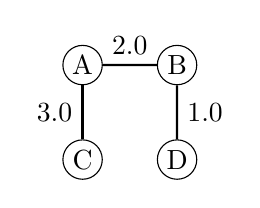
\begin{tikzpicture}[scale=0.6,place/.style={circle,draw, fill=white,inner sep=0pt,minimum size=5mm}]
        \node (x31)  at (2,2) [place] {B};
        \node (x21)  at (2,0) [place] {D};
        \node (x22)  at (0,0) [place] {C};
        \node (x11)  at (0,2) [place] {A};

        \draw [thick] (x31) -- (x21)
            node[right,text centered,midway]{1.0};
        \draw [thick] (x22) -- (x11)
            node[left,text centered,midway]{3.0};
        \draw [thick] (x11) -- (x31)
            node[above,text centered,midway]{2.0};
        \end{tikzpicture}
        \label{Fig:8_1_B}
    }
    \hfil
    \subfloat[]{
        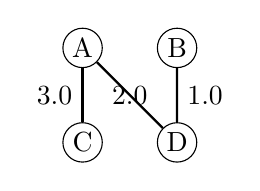
\begin{tikzpicture}[scale=0.6,place/.style={circle,draw, fill=white,inner sep=0pt,minimum size=5mm}]
        \node (x31)  at (2,2) [place] {B};
        \node (x21)  at (2,0) [place] {D};
        \node (x22)  at (0,0) [place] {C};
        \node (x11)  at (0,2) [place] {A};

        \draw [thick] (x31) -- (x21)
            node[right,text centered,midway]{1.0};
        \draw [thick] (x22) -- (x11)
            node[left,text centered,midway]{3.0};
        \draw [thick] (x21) -- (x11)
            node[text centered,midway]{2.0};
        \end{tikzpicture}
        \label{Fig:8_1_C}
    }
    \hfil
    \subfloat[]{
        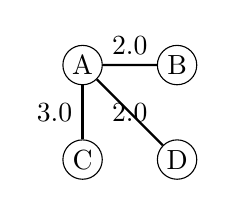
\begin{tikzpicture}[scale=0.6,place/.style={circle,draw, fill=white,inner sep=0pt,minimum size=5mm}]
        \node (x31)  at (2,2) [place] {B};
        \node (x21)  at (2,0) [place] {D};
        \node (x22)  at (0,0) [place] {C};
        \node (x11)  at (0,2) [place] {A};

        \draw [thick] (x22) -- (x11)
            node[left,text centered,midway]{3.0};
        \draw [thick] (x11) -- (x31)
            node[above,text centered,midway]{2.0};
        \draw [thick] (x21) -- (x11)
            node[text centered,midway]{2.0};
        \end{tikzpicture}
        \label{Fig:8_1_D}
    }
    \caption{一个图和它的一些生成树:其中两个是最小生成树。}
    \label{Fig:8_1}
\end{figure*}

有很多情况必须找最小生成树。无论什么时候想找最便宜的方式连接一些终端站点。
比如城市、电子终端、计算机、工厂使用路,电线或是电话线,解决的方法都是找
最小生成树,其中边是所有可能的连接,权是可能连接的花费。找最小生成树也是
各种路由算法的重要子问题,即访问图的每一个顶点的有效的路径。

就像图\ref{Fig:8_1}中展示的简单例子,一个带权图可以有许多最小生成树。
事实上,这个例子中将一个最小生出树转换成另一个的方法在
\ref{Sec:PropertiesOfMST}小节中讨论,这个图是后面讨论最小生成树时一直使用
的图。

\subsection{算法的概况}
因为无向图是连通的,且任意节点都可以认为是根,一个自然的找最小生成树的
想法是每次给起始顶点“增加”一条边。我们必须首先使用标准的遍历算法,
深度优先和广度优先遍历算法。如果我们可以使用其中的一个框架解决这个问题,
则我们就可以在线性时间解决问题,这肯定是最佳的。你必须花点时间尝试使用
这些搜索算法的思想,并构造标准搜索算法不能找到最小的例子(练习8.1)

使我们相信简单的遍历似乎不能解决问题的时候,考虑到这是个最优化问题,
下一个自然的想法使尝试\emph{贪婪}方法。贪婪方法的思想是:不断选择取短期消耗最小
的行动,以期望大量的短期最小消耗加起来得到一个小的总体消耗。(可能的
回溯是指:小的短期消耗可能导致下一步不可避免的会是一个很大的消耗。)我们
会有一个很自然的想法,即在我们增加边的时候增加短期消耗最小的边:简单的
增加可以增加到树的边\footnote{译注:不会将树变成图},且有最小的权。
Prim's算法就是这样一个贪婪实现。

有了解决问题的思路,还有两个问题。它工作正确吗?它运行的有多快?我们
已经提及,一系列短期消耗可能导致到不好的情况,所以即使我们得到一颗生成树,
我们还需要考虑它的权是不是所有生成树中最小的。同样,既然我们需要在
每一步都从每一条边中选一条,而且候选集合在每一步之后都会变,我们需要
选一种数据结构使得这些操作比较高效率。在解决了通用思想后,我们将回到
这些问题。

Prim's算法开始要任意的选一开始顶点,在通过不断选出新的顶点和边“分支出”树
的部分。新边连接新的顶点到前面生成的树。在整个算法过程中,顶点可以划分成
3个不相交的集合:
\begin{enumerate}
\item \emph{树}的顶点:当前在树中的,
\item \emph{边缘}的顶点:不在树中,但是与树中的顶点邻接,
\item \emph{没有检查}的顶点:剩下的全部。
\end{enumerate}

算法关键的步骤是从边缘顶点中选一个顶点和附带边。实际上,因为权是边的权,
选择的焦点在边,不在顶点。Prim's算法总是选择最小权的从树的顶点到边缘
的顶点的边。算法的一般结构如下:

\begin{lstlisting}[language={Java}, keywordstyle=\color{blue!70}, commentstyle=\color{red!50!green!50!blue!50}]
primmest(G, n)
    `初始化所有的顶点为没有检查。`
    `选择任意顶点s开始树;将它划分到\emph{树}。`
    `划分所有与s邻接的顶点为\emph{边缘}。`
    `当有边缘顶点时:`
        `选择一条权最小的从树顶点t到边缘顶点v的边;`
        `将v划分到\emph{树};添加边tv到树;`
        `将所有与v邻接的边缘顶点划分到\emph{没有检查}的顶点。`
\end{lstlisting}

\begin{figure*}[!t]
    \centering
    \subfloat[带权图]{
        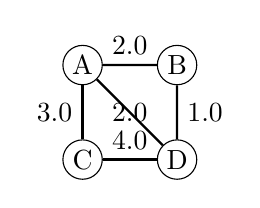
\begin{tikzpicture}[scale=0.6,place/.style={circle,draw, fill=white,inner sep=0pt,minimum size=5mm}]
        \node (x31)  at (2,2) [place] {B};
        \node (x21)  at (2,0) [place] {D};
        \node (x22)  at (0,0) [place] {C};
        \node (x11)  at (0,2) [place] {A};

        \draw [thick] (x31) -- (x21)
            node[right,text centered,midway]{1.0};
        \draw [thick] (x21) -- (x22)
            node[above,text centered,midway]{4.0};
        \draw [thick] (x22) -- (x11)
            node[left,text centered,midway]{3.0};
        \draw [thick] (x11) -- (x31)
            node[above,text centered,midway]{2.0};
        \draw [thick] (x21) -- (x11)
            node[text centered,midway]{2.0};
        \end{tikzpicture}
        \label{Fig:8_2_A}
    }
    \hfil
    \subfloat[开始选择时树和边缘顶点]{
        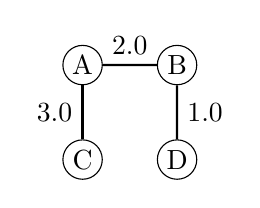
\begin{tikzpicture}[scale=0.6,place/.style={circle,draw, fill=white,inner sep=0pt,minimum size=5mm}]
        \node (x31)  at (2,2) [place] {B};
        \node (x21)  at (2,0) [place] {D};
        \node (x22)  at (0,0) [place] {C};
        \node (x11)  at (0,2) [place] {A};

        \draw [thick] (x31) -- (x21)
            node[right,text centered,midway]{1.0};
        \draw [thick] (x22) -- (x11)
            node[left,text centered,midway]{3.0};
        \draw [thick] (x11) -- (x31)
            node[above,text centered,midway]{2.0};
        \end{tikzpicture}
        \label{Fig:8_2_B}
    }
    \hfil
    \subfloat[在选择一条边和顶点之后:BG没有画出,因为AG是到达G更好的选择(有更低的权)]{
        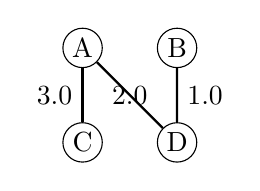
\begin{tikzpicture}[scale=0.6,place/.style={circle,draw, fill=white,inner sep=0pt,minimum size=5mm}]
        \node (x31)  at (2,2) [place] {B};
        \node (x21)  at (2,0) [place] {D};
        \node (x22)  at (0,0) [place] {C};
        \node (x11)  at (0,2) [place] {A};

        \draw [thick] (x31) -- (x21)
            node[right,text centered,midway]{1.0};
        \draw [thick] (x22) -- (x11)
            node[left,text centered,midway]{3.0};
        \draw [thick] (x21) -- (x11)
            node[text centered,midway]{2.0};
        \end{tikzpicture}
        \label{Fig:8_2_C}
    }
    \caption{Prim's算法一次迭代之后:实线表示树的边,虚线表示到边缘顶点的边。}
    \label{Fig:8_2}
\end{figure*}

\begin{example}
Prim's算法,一次迭代

图\ref{Fig:8_2_A}展示了一个带权图。假设A是开始的顶点。循环开始之前的步骤
导致到图\ref{Fig:8_2_B}。在第一次循环的迭代之后,边缘顶点中的最小权边是AB。
因此B被添加到树,与B邻接的没有检查顶点划分到边缘顶点,导致了图\ref{Fig:8_2_C}。
\end{example}

我们能确定这个策略会导致一个最小生成树吗?在短期贪婪的策略是一个好的长期
策略吗?在这种情况,是。下两个小节讨论所有最小生成树的公共特性,使用这些
特性展示Prim's算法每一步构造的树都是这颗树的子图上的最小生成树。在
\ref{Sec:8_2_5}小节我们将讨论实现的问题。

\subsection{最小生出树的属性}\label{Sec:PropertiesOfMST}
图\ref{Fig:8_1}展示了一个带权图可能有多个最小生成树。事实上,最小生成树
有一个公共特性,用这个特性我们可以将一颗最小生成树一步一步转换成另一颗
最小生成树。考察这些特性也有助于我们更熟悉无向树(also help us to become
 more familiar with undirected trees, generally)。

\begin{definition}
最小生成树特性

给出连通带权图$G=(V, E, W)$,令$T$是$G$的任意生成树。假设$G$的每一条不在
$T$中的边$uv$,如果$uv$增加到$T$,使得产生了一个回路,而$uv$是这个回路中
权最大的边。则树T有最小生出树属性(简称为MST属性)。
\end{definition}

首先,让我们看看定义的意思。之后我们将证明这个名字是
很恰当的\footnote{译注:即符合这一特性的确实是最小生成树};仅仅是叫
“最小生成树属性”并不意味着可以不作任何事情就说它是最小生成树!

\begin{example}
最小生成树属性

根据定义一颗无向树连接树中的任意两个顶点,且没有环。图\ref{Fig:8_1}就是
一个简单图,我们称之为$G$,还有3颗生成树。首先另$T$是\ref{Fig:8_1_B}代表
的树。假设我们增加一条$G$的不属于$T$的边到$T$上,得到新图$G_1$(我们将增加
权值是2的那条)。这产生了一个回路($G_1$中唯一的回路)。(为什么呢?
\footnote{译注:生成树两个顶点间必然有一条路径,增加一条不属于生成树的路径,
必然和生成树中的路径构成回路})回路中其他的边的权值最多是2,即不超过加入边
的权值。可选的,如果我们加入权值4的边,则回路中其他边的权值最多是4(事实
上是4)。这里只有两条可选的边,所以$T$有最小生成树属性。\ref{Fig:8_1_C}代表
的树也是一样。

但是,现在考虑令$T$是让\ref{Fig:8_1_D}代表的树,增加权值1的边。这次回路中
有些边的权值就超过1了。因此\ref{Fig:8_1_D}代表的树不符合最小生成树属性。
注意我们可以去掉回路中任意一条边得到新图$G_2$,$G_2$也必然是一颗树,事实上
还是一颗生成树。在练习8.2中证明了这个事实,这个事实用于证明下面的引理和定义。
既然有一条边的权值大于1,那么我们选择去掉这条权值大于1的边。这意味着$G_2$的
权值要小于T,所以T不是最小生成树。
\end{example}

\begin{lemma}\label{Lemma:8_1}
在一个连通,带权图$G=(V, E, W)$中,如果$T_1$和$T_2$是两颗符合MST属性的生成树,
则他们有相同的权。

{\textbf{\emph{证明}}} 令$k$是在$T_1$中但是不在$T_2$中的边的数目,证明用归纳$k$
的方式。(在$T_2$中不在$T_1$中的边的数目$k$也是类似的。)基本情况是$k=0$;在
这种情况下,$T_1$和$T_2$是相同的,所以他们有相等的权。

对于$k>0$,令当0到$k-1$条边都不同时,引理是符合的,则当有$k$条边不同时。令$uv$
是在$T_1$中或$T_2$中但是不同时在两者中的最小权的边。假设$uv\in T_2$;$uv\in T_1$
是等价的。考虑$T_1$中$u$到$v$唯一的路径:$w_0, w_1, \cdots, w_p$,这里$w_0=u$,
$w_p=v$,$p\geq 2$。这条路径必然包含有不在$T_2$中的边。(为什么?
\footnote{译注:因为$uv\in T_2$,如果$T_1$中$u$到$v$的边都在$T_2$中,则$T_2$中
存在两条从$u$到$v$的路径,与$T_2$是树的属性不符。$p$必须不小于2是同样的道理。})
令$w_iw_{i+1}$就是这样的边。由$T_1$的MST属性知,$w_iw_{i+1}$的权不大于$uv$的权。
但由于$uv$是不同时在$T_1T_2$的权最小的边,所以$w_iw_{i+1}$的权不小于$uv$的权。
因此$W(w_iw_{i+1})=W(uv)$。增加$uv$到$T_1$形成回路,则移出$w_iw_{i+1}$,打开回路,
得到新的生成树$T_1'$,新的生成树与$T_1$有相同的权。但是$T_1'$与$T_2$仅有$k-1$条边
不一样,由于归纳假设,两者有相同的权,因此$T_1$和$T_2$有相同的权。
\end{lemma}

引理的证明也向我们展示了一种一步一步将任何最小生成树$T_1$转换成另一颗最小生成树$T_2$
的方法。选择一条$T_2$中但不在$T_1$中权最小的边$uv$。找到$T_1$中$u$到$v$的路径。
路径中肯定有一条不在$T_2$中但权与$uv$相等的边,$xy$。(参见练习8.3)移出$xy$增加$uv$。
这样就朝$T_2$前进了一步。重复,直到得到$T_2$。

\begin{theorem}
在连通带权图$G=(V, E, W)$,树$T$是最小生成树当且仅当$T$有MST属性。

{\textbf{\emph{证明}}} (仅当)假设$T$是$G$的最小生成树。假设存在一条不在$T$中的边$uv$,
将$uv$添加到$T$之后构成回路,回路中有另一条边$xy$使得$W(xy)>W(uv)$。则移出$xy$得到新的
生成树,新的生成树的权小于$T$,与$T$是最小生成树的假设矛盾。

(当)假设$T$有MST属性。令$T_{min}$是$G$的任意最小生成树。由前面的证明可知$T_{min}$有
MST属性。由引理\ref{Lemma:8_1},$T$和$T_{min}$有相同的权。

\end{theorem}

\subsection{Prim's MST算法的正确性}
我们现在使用MST属性来展示Prim's算法确实构造了一颗最小生成树。这个证明用了一种
在采用归纳时经常出现的形式:通过归纳证明的语句有时比我们感兴趣的定理更详细。
所以我们首先将这更详细的语句作为引理证明。之后定理简单的吸取引理感兴趣的部分。
以这种观点,定理非常象递归过程的“包装”,就像3.2.2小节讨论的。

\begin{lemma}
令G=(V, E, W)是连通的带权图,$n=|V|$;令Tk是一个由Prim's算法创建的有k个顶点的树,
其中$k=1, \cdots, n$;令$G_k$是G中$T_k$的顶点组成的子图(例如,uv是$G_k$
的一条边,当这条边在G中,且u、v都在$T_k$中。)则在$G_k$中$T_k$有MST属性。

{\textbf{\emph{证明}}} 证明是对k的归纳。基本情况是k=1。这种情况下,$G_1$和
$T_1$仅包含起始节点s没有边, 所以在$G_1$中$T_1$有MST属性。

对于$k>1$时,假设对于$1 \leq j < k$都有在$G_j$中$T_j$有MST属性。假设Prim's算法
加入增加到树中的第k个顶点是v,v到$T_{k-1}$中顶点的边分别是$u_1v, \cdots, u_dv$。
For definiteness,假设$u_1v$是最小的边,因此被算法选中。我们需要验证$T_k$有
MST属性。就是说,如果xy是任意在$G_k$中但不在$T_k$的边,则将xy加入$T_k$中后形成
的回路中xy是权最大的边。如果$x\neq v$且$y\neq v$,则xy也在$G_{k-1}$中,但是不在
$T_{k-1}$中,所以根据归纳假设,它增加到$T_{k-1}$之后是回路中权最大的边。但是
这个回路同样是$T_k$的回路,所以这种情况下$T_k$也有MST属性。剩下的就是检查xy是
$u_2v, \cdots, u_db$其中一条时(因为$u_1v$已经在$T_k$中了)。对于$d<2$时我们
已经作了,现在假设$d\geq 2$。

引用图8.3会在剩下的证明中帮助我们的。考虑v到$T_k$中$u_i$路径,对于任意i,
$2 \leq i \leq d$。假设这些路径上存在边的权大于$u_iv$的权,至少有$u_1v$的权
(如果不存在,MST属性就满足了。)特别的,令路径是$v, w_1, \cdots, w_p$,这里
$w_1=u_1$且$w_p=u_i$。则$w_1, \cdots, w_p$是$T_{k-1}$中的路径。令$w_aw_{a+1}$是
路径中第一条权比$W(u_iv)$大的边,令$w_bw_{b+1}$是路径中最后一条权比$W(u_iv)$大
的边(可能a+1=b;看图8.3)。我们认为如果$w_a$和$w_b$是由Prim's算法构造的话,则
$w_a$和$w_b$不能存在于$T_{k-1}$。假设$w_a$在$w_b$之前加入树。则从$w_1$(就是$u_1$)
到$w_a$的路径上所有的边将在$w_aw_{a+1}$和$w_bw_{b+1}$之前被加入,因为他们有更小
的权,且$u_1v$也将在他们之前加入。类似的,如果$w_b$在$w_a$之前加入树,则$u_iv$也
将在$w_aw_{a+1}$或$w_bw_{b+1}$之前加入。但是$u_1v$或者$u_iv$都不在$T_{k-1}$中,
所以$w_1, \cdots, w_p$中没有边的权大于$W(u_iv)$,$T_k$符合MST属性。
\end{lemma}

\begin{theorem}
Prim's算法输出最小生成树

证明 在引理8.3的术语中,$G_n=G$和$T_n$是算法的输出,所以$T_n$在$G$中有MST属性。
由定理8.2知,$T_n$是$G$的最小生成树。
\end{theorem}

\subsection{用优先权队列有效的管理边缘}\label{Sec:8_2_5}
在算法循环的每一个迭代之后,就可能有新的边缘顶点,而且下一次待选择的边集合也会
改变。图8.2(c)建议我们需要考虑树的顶点和边缘顶点之间所有的边。在选择AB之后,BG成
了一个待选项,但是要丢弃BG因为AG的权值比BG低,AG将是到达G的更好的选择。如果BG的
权值比AG低,则丢弃AG。对于每一个边缘顶点,我们需要保持到树的一条边即可:权值最小
的那条。我们称这样的边为\emph{候选边(candidate edges)}。

优先权队列ADT(2.5.1小节)恰好有我们实现8.2.2小节算法所需要的操作。Insert操作
加入一个顶点到优先权队列。getMin操作可以用于选取边缘顶点,

使用优先权队列ADT操作,高层算法如下。一个子例程updateFringe用来处理顶点邻接

\subsubsection{初步分析}
在不知道优先权队列是如何实现时,我们能算法的运行时间吗?第一步是求出每一个ADT
操作消耗多少时间。然后我们可以写出表达式。

\subsection{实现}
算法主要的数据结构(除了图本身以外)
\subsection{分析(时间和空间)}
我们现在完成了算法8.1在G=(V,E,W)的分析。

\subsection{The Pairing Forest Interface}
\subsection{底限}
到底找到最小生成树需要多少工作?我们宣称任何一个最小生成树算法在最坏情况下需要
$\Omega(m)$,因为它必须以某种方式处理图的每一条边。令G是一个连通的带权图,每一条
边至少有权值2,并假设有一个算法对G中的边xy完全不做任何事情。则xy肯定不在算法输出
的树T中。将xy的权改为1。这可能不改变算法的行为,因为算法不检查xy。但是由定理8.2知,
现在T不再符合MST属性,它不再是一颗最小生成树。事实上,为了得到一颗更“轻”的树,
只需要简单的xy加入T中,然后移除回路中的另一条边就可以了。因此算法不检查xy是错误的。

\section{单源最短路径}\label{Sec:single-source-shortest-path}
在7.2小节中我们简要的考虑了在航空路线图上如何找到两个城市间最好的路线的问题,
比如图7.8。使用的标准是我们关心的机票的价格,我们观察最好的--就是说最便宜的--从
San Diego到Sacramento的方式是在Los Angeles中转一下。这是一个非常普通的带权图
的问题的实例,或叫应用:在两个特定的顶点之间找到最小权的路径。

最坏情况下,基本上成了两个问题:找到一对特定顶点s和t之间的最小权路径;找到
从s到每一个可以从s到达的顶点的最小权路径。这两个问题一样的复杂。后一个问题叫
做单源最短路径问题。两者采用同样的算法。

本节考虑在带权有向图和无向图上找从一个源顶点到每一个其他顶点最小权路径的问题。
路径的权(长度或是耗费)是路径上所有边的权的和。当权被解释成距离时,一个最小权
路径叫做最短路径,而且这是最常用的名字。(唉,它混合了术语权,耗费和长度。)

我们是如何确定图7.4中SD到SAC的最短路径的呢?事实上,对于这个简单的例子我们使用
了很不规则的方法,充满了假设,比如城市之间的费用和距离是成比例的,地图是按比例
精确画的。则我们捡了一条看上去短的路线,然后加起来了耗费。最后,我们检查了许多
其他的路线(somewhat haphazardly)没有注意到有改进,所以我们宣布问题解决了。这是
一个很难用于计算机编程的算法。我们发现这确实能诚实的回答上面的问题;人们一般
使用非常不严格的方式来解决问题,特别是对非常小的数据集合。

实践中,当V中包含上百,上千,甚至百万个顶点的时候,在图中找最短路径的问题就麻烦
了。理论上算法必须考虑所有可能的路径而且比较他们的权值,但是实践中这可能需要很长
的时间,可能有几个世纪。为了尝试找到更好的方法,找到最短路径的一些通用的性质是
很有帮助的,然后再来看他们是否能发现一个更有效的方法。我们展示的算法是
E.W.Dijkstra提出的。这个算法需要边的权都是非负的。其他一些不需要这个限制的算法
在本章后面的Notes和References中提到。



\subsection{最短路径的属性}
一般的,当尝试解决一个大问题的时候,我们想把它分解成小的问题。What can we say
about shortest paths between distant nodes, in terms of shortest paths between
less distant nodes? 我们可以使用某种形式的分而治之方法吗?假设路径P是x到y的
最短路径而Q是y到z 的最短路径。那么是否意味着P接上Q就是x到z的最短路径?不用很长
的时间就可以找出一个例子来说明它不对。但是它的逆命题是对的。下面的引理的证明留到
练习中。

\begin{lemma}
(最短路径的属性)在带权图G中,假设x到y的最短路径由从x到y的路径P和从y到z的
路径Q组成。则P是x到y的最短路径,Q是y到z的最短路径。
\end{lemma}

假设我们要尝试找x到z的最短路径。可能一条直接的边xz存在,且提供了最短的路径。但是,
如果最短的路径包含2条或更多的边,则引理告诉我们它可以被分解成两条路径,每一条比
原来包含的边少,每一条都是自己的最短路径。为了发展这个算法,我们需要建立一些分解路径
的有组织的方案。

\subsection{Dijkstra's最短路径算法}\label{Sec:Dijkstra}
本小节中我们学习Dijkstra's最短路径算法;它非常类似与前一小节的Prim's最小生成树算法。

\begin{definition}\vspace{1ex}
令P是一条带权图上G=(V, E, W)上的非空路径,由k个边$xv_1, v_1v_2, \cdots, v_{k-1}y$
(可能$v_1=y$)。P的权,表示为$W(p)$是权$W(xv_1), W(v_1v_2), \cdots, W(v_{k-1}y)$。
如果x=y,认为x到y有空路径。空路径的权是0。

如果x到y没有路径的权小于$W(p)$,则P称为最短路径,或是最小权路径。
\end{definition}

前面的定义小心的表达了负权的可能性。但是,在本节中我们假定权是非负的。在这个限制下,
最短路径可以限制成一条简单路径。

\begin{problem}
单源最短路径

给出带权图G=(V, E, W)和一个源顶点s。问题是找出s到每一个顶点v的最短路径。
\end{problem}

在开始之前,我们必须考虑我们是否需要一个全新的算法。假设我们使用最小生成树的算法,
从s开始。由算法构造的树中到v的路径是否就是s到v的最短路径?考虑图8.4中最小生成树
中A到C的路径。它不是最短路径;路径A,B,C更短。

Dijkstra's最短路径算法通过增加到s的距离来找s到其他顶点的最短路径。算法,类似于
8.2小节的Prim's MST算法,从一个顶点(s)开始,通过选择到新顶点的特定的边来“向外分支”。
由算法生成的树叫最短路径树。(叫这个名字不意味着它就是;必须证明在树中的路径
确实是最短路径。)

同样类似于Prim's MST算法。Dijkstra's算法是贪婪算法;它总是选择出现的“最近”的
顶点的边;但是这里的“最近”是到s最近,而不是“到树最近”。顶点被分成3(不相交)
部分如下:
\begin{enumerate}
\item \emph{树}的顶点:当前在树中的,
\item \emph{边缘}的顶点:不在树中,但是与树中的顶点邻接,
\item \emph{没有检查}的顶点:剩下的全部。
\end{enumerate}
同Prim's算法一样,我们记录唯一的到边缘顶点的候选边(当前找到最好的)。对每一个
边缘顶点z,这里至少有一个树中的顶点v,使得vz是G的一条边。对于每一个这样的v都有
(唯一的)树中的从s到v的路径(可能s=v);d(s, v)表示路径的权。添加一条边vz到
这条路径,,得到s到z的路径,它的权是d(s,v)+W(vz)。z的候选边是vz,因为d(s,v)+W(vz)
是当前所有树中颗选择顶点最小的。

\begin{example}
最短路径树的增长

看图8.9(a)的图。每一个无向边都被看作是……………………………………….
\end{example}

Dijkstra's 算法的一般结构如下:\\
dijkstraSSSP(G,n)\\
\indent    初始化所有的顶点为\emph{没有检查}。\\
\indent     从指定的源顶点s开始树;将其作为树的根;\\
\indent     定义d(s,s)=0。\\
\indent     将所有邻接的顶点划成\emph{边缘}。\\
\indent     当还有边缘顶点时:\\
\indent \indent         在树的顶点t和边缘顶点v中选择一条边,使得d(s,t)+W(tv)最小;\\
\indent \indent         将v划到\emph{树}顶点;将边tv添加到树;\\
\indent \indent         定义d(s,v)=(d(s,t)+W(tv))。\\
\indent \indent         将所有邻接v的\emph{没有检查}顶点划成\emph{边缘}顶点。\\

因为d(s,y)+W(yz)作为候选边可能重复使用,它可以被计算一次并保存。为了有效的计算
它当yz第一次变成候选边时,我们也为树中的每一个y保存d(s,y)。因此我们可以使用
数组dist:
\begin{lstlisting}[language={Java},keywordstyle=\color{blue!70}, commentstyle=\color{red!50!green!50!blue!50}]
    dist[y]=d(s,y);          //`树中的y`
    dist[z]=d(s,y)+W(yz);    //`对于在边缘的z,yz是z的候选边`
\end{lstlisting}
就像在Prim's算法中,在一个顶点和相应的候选边被选择之后,在数据结构中的信息
必须为某些边缘顶点和以前的没有检查顶点更新。

\begin{example}
更新距离信息

在图8.9(d)中……………….
\end{example}

这个方法正确吗?关键的步骤是选择下一个边缘顶点和候选边。对于任意候选边
yz,d(s,y)+W(yz)并不必须是s到z的最短距离,因为到z的最短路径可能不穿过y。
(例如在图8.9中,到H的最短路径并不经过G,尽管GH是c,d和e的可选的一部分。)我们
认为,如果d(s,y)是每一个树顶点y的最短距离,在所有候选边中选出最小的d(s,y)+W(yz)
从而选出了yz,则yz就是给出的最短路径。这个观点在下面的定理中证明。

\begin{theorem}
令$G=(V, E, W)$是一个带非负权的图。令V`是V的一个子集,令s是V`是的成员。假设d(s,y)
是G中s到每一个$y\in V'$的最短的距离。如果为了使d(s,y)+W(yz)最小选择边yz,
其中y在V`中,z在V-V`中,则由s到y的最短的路径更上yz就是s到z的最短路径。

{\textbf{\emph{证明}}} 看图8.10。假设e=yz被选择,令$s, x_1, \cdots, x_r, y$是s到y的最短路径
(可能y=s)。令$P=s, x_1, \cdots, x_r, y, z$。W(P)=d(s,y)+W(yz)。令
$s, z_1, \cdots, z_\alpha, \cdots, z$是s到z的最短路径;叫$P'$。顶点$z_\alpha$
是$P'$中不在$V`$中的第一个顶点(可能za=z)。我们必须说明$W(p)\leq W(P')$。
(如果$a=1$,$z_0=s$,算法将选择$z_{\alpha-1}z_\alpha$。)因为选择了e
\begin{equation}
    W(P)=d(s,y)+W(e)\leq d(s,z_{\alpha-1})+W(z_{\alpha-1}z_\alpha)
\end{equation}
由于引理8.5,$s, z_1, \cdots, z_{\alpha-1}$是s到$z_{\alpha-1}$的最短路径,
所以这条路径的权是$d(s, z_{\alpha-1}$ 。既然$s, z_1, \cdots, z_{\alpha-1}, z_\alpha$
是$P'$的一部分,且每条边都是非负的,
\begin{equation}
d(s, z_{\alpha-1})+W(z_{\alpha-1}z_\alpha)\leq W(p')
\end{equation}
联合(8.2)(8.3),$W(p)\leq W(P')$。
\end{theorem}

\begin{theorem}
给出一个带非负权的图G和源顶点s,Dijkstra's算法计算出s到G中每一个可到达顶点
的最短距离(最小权的路径的权)。

证明 通过将顶点不断加到最短路径树的序列来证明。细节留到8.16中。
\end{theorem}

\subsection{实现}
\subsubsection{分析}
对于8.2.7小节对Prim's最小生成树算法,算法8.1,的分析可以不做任何改变搬到对Dijkstra's
最短路径算法,算法8.2,上来。Dijkstra's算法在最坏情况下也运行在$\Theta(n^2)$。
同样的低限$\Omega(m)$,空间需求也是$\Theta(n)$。

如果不可到达顶点的数量很多,则预处理的时候测试可到达性会更有效率,消除不可
到达顶点,对可到达的重新编号$1, \cdots, n_r$。总的消耗是$\Theta(m+n_r^2)$,
而不是$\Theta(n^2)$。


\section{Kruskal's 最小生成树算法}\label{Sec:KruskalMST}
令$G=(V, E, W)$是有向带权无向图。\ref{Sec:PrimMST}节中我们学习了找图G最小生成树的
Prim's算法(G必须是连通图)。算法从任意顶点开始,通过“贪婪的”选择最小
权的边不断分支出树。任何时候加入一条边都是一颗树。这里我们检查另一种用
贪婪策略的算法。本节中所有的图都是无向图。

\subsection{算法}
Kruskal's算法的一般思想如下。每一步它都在图剩下的边中选一条权最小的,但是
丢弃与已选择的边构成回路的。任意时刻选择的边都可能相距很远,使得形成森林,而
不必须是树。当所有边都处理过之后算法终结。
\begin{figure}
\begin{lstlisting}[language={Java},keywordstyle=\color{blue!70}, commentstyle=\color{red!50!green!50!blue!50}]
    kruskalMST(G, n)
    {
        R=E;
        F=`空集合`;
        while(R`非空`)
        {   `移除R中权最小的边,比如vw`;
            if(`vw不在F中形成回路`)
                `添加vw到F`;
        }
        return F;
    }
\end{lstlisting}
\end{figure}
在考虑如何实现这个思想之前,我们必须问它是否能工作。既然图可以不是连通的,
我们首先需要一个定义。

\begin{definition}
生出树集合

令G=(V, E, W)是带权无向图。G的\emph{生出树集合}是一个树的集合,每一棵树都是G的
一个连同分量,集合中的树都是连同分量的生成树。\emph{最小生成树集合}是生成树集合
中,边权的和最小的生成树的集合,就是说是最小生成树的集合。
\end{definition}

首先,G的每一个顶点都在某棵树中吗(如果图是非连通的,就可能有多棵树)?令v
是G的任一顶点。如果至少一条边连在v上,令S是附加在v上所有边的集合,则第一条
从S中取走的边将加入F。但是如果v是孤立顶点(没有边与之相连),则它将不出现在
F中,而且没有忽略它的话,需要单独考虑。

下一个问题是算法生成的是否是生成树集合,假设G没有孤立顶点。就是说,对G的每一个
连通分量F中是否都有一棵精确的树?下面的引理提供了这个问题的一些理解。证明
是简单的,留在练习中。

\begin{lemma}
令F是森林;就是任意无向无环图。令e=vw是不在F中的边。如果e和F中的边构成回路,
当且仅当v和w属于F的同一个连通分支。
\end{lemma}

现在假设G的有些连通分量对应Kruskal's算法得到的森林F中的两棵或两棵以上的树。
G中必然存在边连接这两颗树,称为vw;v和w属于F不同的连通分支。因此,当算法
处理边vw时,它必然会得到F',F'在森林中有回路存在。所以vw不会添加到F'。
由于引理8.8,v和w

\subsection{分析}
